\documentclass[14pt]{extbook}
\usepackage{multicol, enumerate, enumitem, hyperref, color, soul, setspace, parskip, fancyhdr} %General Packages
\usepackage{amssymb, amsthm, amsmath, latexsym, units, mathtools} %Math Packages
\everymath{\displaystyle} %All math in Display Style
% Packages with additional options
\usepackage[headsep=0.5cm,headheight=12pt, left=1 in,right= 1 in,top= 1 in,bottom= 1 in]{geometry}
\usepackage[usenames,dvipsnames]{xcolor}
\usepackage{dashrule}  % Package to use the command below to create lines between items
\newcommand{\litem}[1]{\item#1\hspace*{-1cm}\rule{\textwidth}{0.4pt}}
\pagestyle{fancy}
\lhead{Module5}
\chead{}
\rhead{Version B}
\lfoot{3697-2165}
\cfoot{}
\rfoot{test}
\begin{document}

\begin{enumerate}
\litem{
Solve the radical equation below. Then, choose the interval(s) that the solution(s) belongs to.\[ \sqrt{-21 x^2 - 40} - \sqrt{71 x} = 0 \]\begin{enumerate}[label=\Alph*.]
\item \( x \in [-4.7,-2.1] \)
\item \( x \in [-0.8,0.7] \)
\item \( x_1 \in [-4.7, -2.1] \text{ and } x_2 \in [-2.3,0.5] \)
\item \( x_1 \in [0.7, 5.3] \text{ and } x_2 \in [0.4,2.3] \)
\item \( \text{All solutions lead to invalid or complex values in the equation.} \)

\end{enumerate} }
\litem{
What is the domain of the function below?\[ f(x) = \sqrt[8]{9 x - 6} \]\begin{enumerate}[label=\Alph*.]
\item \( [a, \infty), \text{ where } a \in [0.1, 1.3] \)
\item \( [a, \infty), \text{where } a \in [0.7, 1.9] \)
\item \( (-\infty, a], \text{where } a \in [0.63, 0.78] \)
\item \( (-\infty, \infty) \)
\item \( (-\infty, a], \text{where } a \in [1.18, 1.52] \)

\end{enumerate} }
\litem{
Choose the equation of the function graphed below.
\begin{center}
    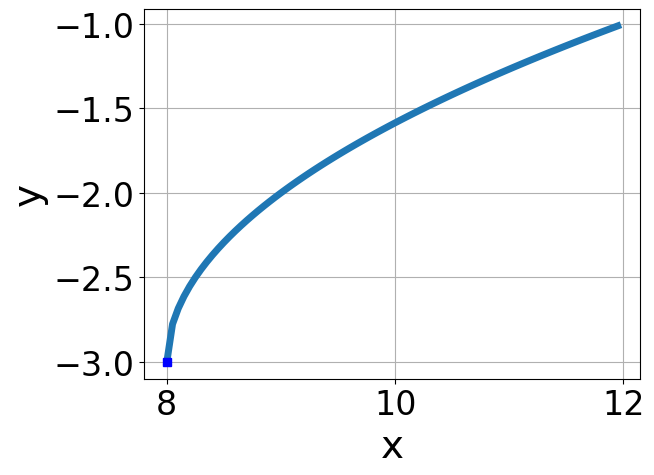
\includegraphics[width=0.5\textwidth]{../Figures/radicalGraphToEquationB.png}
\end{center}
\begin{enumerate}[label=\Alph*.]
\item \( f(x) = - \sqrt[3]{x + 8} - 3 \)
\item \( f(x) = - \sqrt[3]{x - 8} - 3 \)
\item \( f(x) = \sqrt[3]{x - 8} - 3 \)
\item \( f(x) = \sqrt[3]{x + 8} - 3 \)
\item \( \text{None of the above} \)

\end{enumerate} }
\litem{
Solve the radical equation below. Then, choose the interval(s) that the solution(s) belongs to.\[ \sqrt{-36 x^2 - 18} - \sqrt{-51 x} = 0 \]\begin{enumerate}[label=\Alph*.]
\item \( x_1 \in [-0.86, -0.64] \text{ and } x_2 \in [-1.75,0.25] \)
\item \( x \in [0.73,0.8] \)
\item \( x_1 \in [0.57, 0.68] \text{ and } x_2 \in [-0.25,4.75] \)
\item \( x \in [0.57,0.68] \)
\item \( \text{All solutions lead to invalid or complex values in the equation.} \)

\end{enumerate} }
\litem{
Choose the equation of the function graphed below.
\begin{center}
    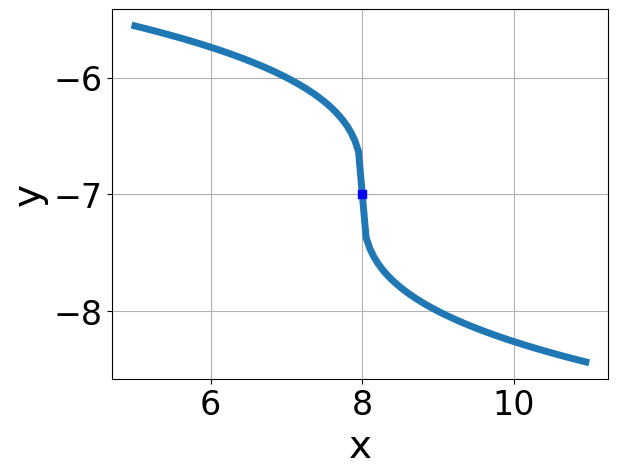
\includegraphics[width=0.5\textwidth]{../Figures/radicalGraphToEquationCopyB.png}
\end{center}
\begin{enumerate}[label=\Alph*.]
\item \( f(x) = - \sqrt[3]{x - 8} - 7 \)
\item \( f(x) = \sqrt[3]{x - 8} - 7 \)
\item \( f(x) = - \sqrt[3]{x + 8} - 7 \)
\item \( f(x) = \sqrt[3]{x + 8} - 7 \)
\item \( \text{None of the above} \)

\end{enumerate} }
\litem{
What is the domain of the function below?\[ f(x) = \sqrt[5]{-5 x - 8} \]\begin{enumerate}[label=\Alph*.]
\item \( \text{The domain is } (-\infty, a], \text{   where } a \in [-0.63, -0.37] \)
\item \( (-\infty, \infty) \)
\item \( \text{The domain is } [a, \infty), \text{   where } a \in [-0.9, -0.2] \)
\item \( \text{The domain is } (-\infty, a], \text{   where } a \in [-3.46, -1.16] \)
\item \( \text{The domain is } [a, \infty), \text{   where } a \in [-2.4, -1.4] \)

\end{enumerate} }
\litem{
Choose the graph of the equation below.\[ f(x) = \sqrt{x - 12} + 5 \]\begin{enumerate}[label=\Alph*.]
\begin{multicols}{2}\item 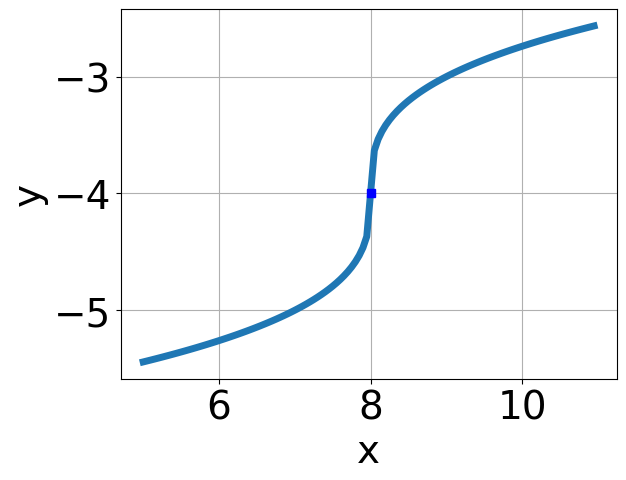
\includegraphics[width = 0.3\textwidth]{../Figures/radicalEquationToGraphAB.png}\item 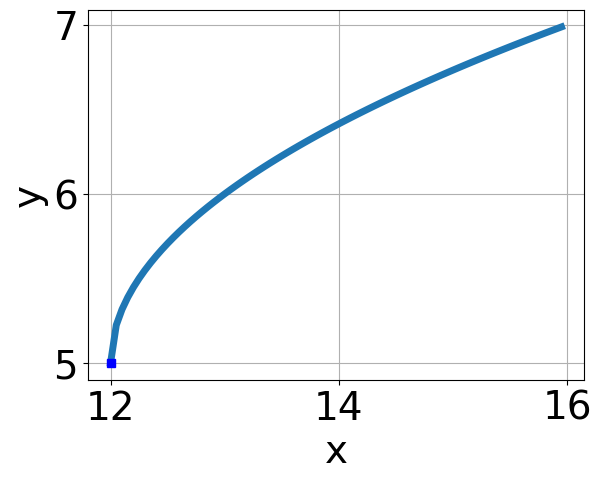
\includegraphics[width = 0.3\textwidth]{../Figures/radicalEquationToGraphBB.png}\item 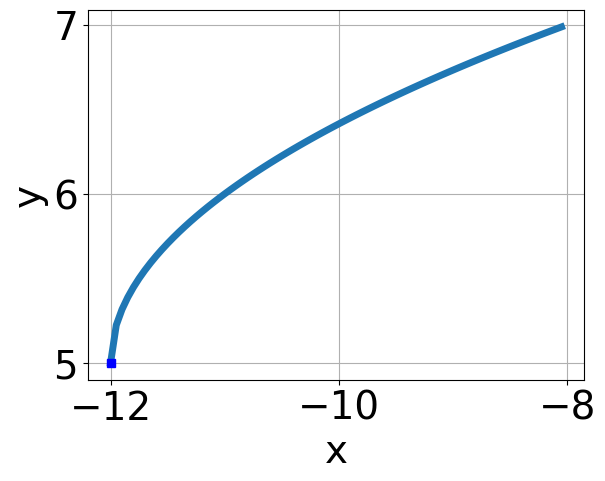
\includegraphics[width = 0.3\textwidth]{../Figures/radicalEquationToGraphCB.png}\item 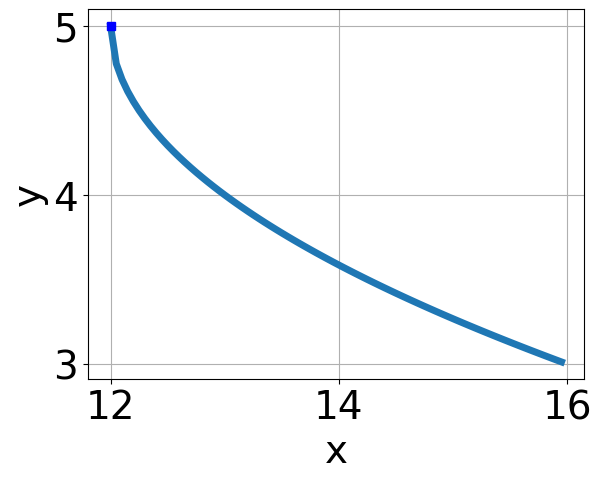
\includegraphics[width = 0.3\textwidth]{../Figures/radicalEquationToGraphDB.png}\end{multicols}\item None of the above.
\end{enumerate} }
\litem{
Solve the radical equation below. Then, choose the interval(s) that the solution(s) belongs to.\[ \sqrt{5 x + 6} - \sqrt{9 x - 7} = 0 \]\begin{enumerate}[label=\Alph*.]
\item \( x_1 \in [-2, -0.3] \text{ and } x_2 \in [-0.4,2.1] \)
\item \( x \in [-0.8,3] \)
\item \( x_1 \in [-2, -0.3] \text{ and } x_2 \in [3.2,5.2] \)
\item \( x \in [1.2,4.8] \)
\item \( \text{All solutions lead to invalid or complex values in the equation.} \)

\end{enumerate} }
\litem{
Choose the graph of the equation below.\[ f(x) = \sqrt[3]{x - 12} + 3 \]\begin{enumerate}[label=\Alph*.]
\begin{multicols}{2}\item 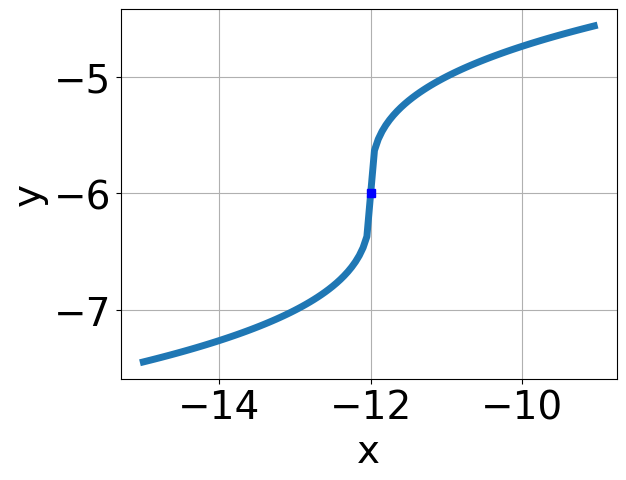
\includegraphics[width = 0.3\textwidth]{../Figures/radicalEquationToGraphCopyAB.png}\item 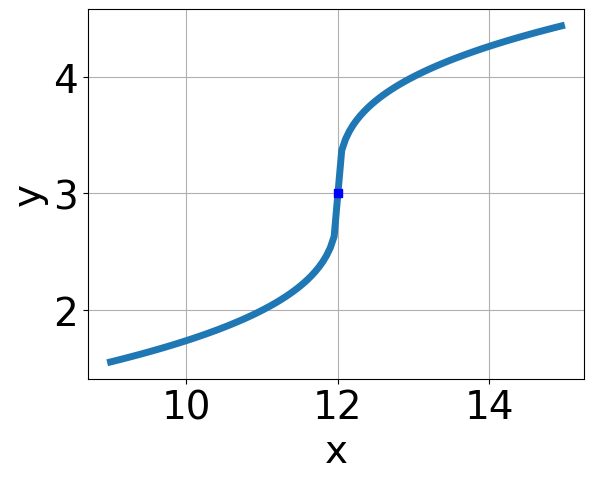
\includegraphics[width = 0.3\textwidth]{../Figures/radicalEquationToGraphCopyBB.png}\item 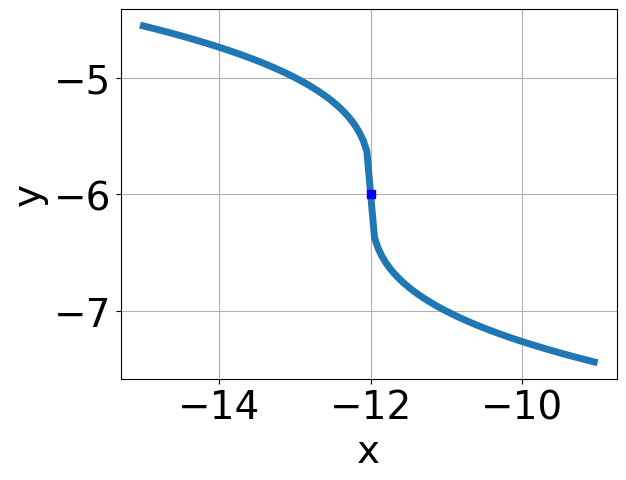
\includegraphics[width = 0.3\textwidth]{../Figures/radicalEquationToGraphCopyCB.png}\item 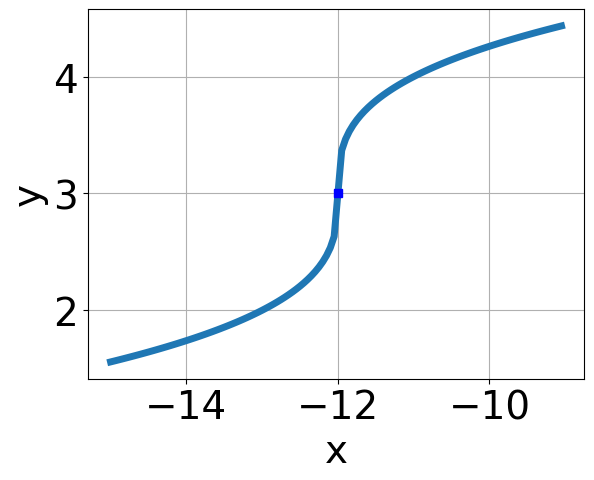
\includegraphics[width = 0.3\textwidth]{../Figures/radicalEquationToGraphCopyDB.png}\end{multicols}\item None of the above.
\end{enumerate} }
\litem{
Solve the radical equation below. Then, choose the interval(s) that the solution(s) belongs to.\[ \sqrt{9 x + 7} - \sqrt{2 x + 3} = 0 \]\begin{enumerate}[label=\Alph*.]
\item \( x_1 \in [-0.8, -0.64] \text{ and } x_2 \in [-0.69,-0.18] \)
\item \( \text{All solutions lead to invalid or complex values in the equation.} \)
\item \( x \in [-1.48,-1.38] \)
\item \( x_1 \in [-1.58, -1.49] \text{ and } x_2 \in [-0.88,-0.69] \)
\item \( x \in [-0.61,-0.45] \)

\end{enumerate} }
\end{enumerate}

\end{document}